\documentclass[a4paper,12pt]{article} %style du document
\usepackage[utf8]{inputenc} %encodage des caractères
\usepackage[french]{babel} %paquet de langue français
\usepackage[T1]{fontenc} %encodage de la police
\usepackage{lmodern} % Police vectorielle
\usepackage[top=2cm,bottom=2cm,left=2cm,right=2cm]{geometry} %marges
\usepackage[pdftex]{graphicx} %paquet d'affichage d'image
\usepackage{makeidx} %paquet d'index
\usepackage{times} %police times new roman
\usepackage{soul} %paquet pour faire des traits
\usepackage{multicol} %environnement multi-colonne


\newcommand{\HRule}{\rule{\linewidth}{1mm}} %commande pour les traits


\makeindex %fait l'index
\begin{document} %début du document
%\pagestyle{headings}


%----------------------------------
%page de garde
%----------------------------------

\begin{titlepage}
\begin{center}

\includegraphics[scale=0.5]{logo-ucbn.png}
\\[3cm]
\Large{Année universitaire 2015-2016}\\[0.5cm]
{\Large \textit{\bfseries {Projet Tuteuré}}}
\\[1cm]
\HRule 
\\[0.4cm]

{\huge {\bfseries {Sujet: Soko'BanZai}}}
\\[0.4cm] 
\HRule\\[1.5cm]

\begin{minipage}{0.4\textwidth}
\begin{flushleft} \large
\emph{\bfseries {Auteurs:}}\\
Guillaume \textsc{Drouart}\\
Marwan \textsc{Lakradi}
\end{flushleft}
\end{minipage}
\begin{minipage}{0.4\textwidth}
\begin{flushright} \large
\emph{\bfseries{Examinateurs:}} \\
Jean-Luc \textsc{Lambert}\\
Bruno \textsc{Zanutinni}
\end{flushright}
\end{minipage}
\vfill
{\large \emph{Diplôme préparé:} ~ L3 Informatique}\\
\end{center}
\end{titlepage}


%------------------------------
%sommaire
%------------------------------

\renewcommand{\contentsname}{Sommaire}
\tableofcontents
\newpage

%-----------------------------
%rédaction
%-----------------------------
\section{Introduction:}
\subsection{Contexte}
Les membres de l'équipe de recherche MAD (Modèles, Agents, Décision) travaillent sur des algorithmes d'intelligence artificielle et souhaiteraient pouvoir les tester sur le jeu Sokoban.
\newline
\subsubsection{Objectifs du projet}
L'équipe de recherche MAD souhaiteraient pouvoir, lors des démonstrations des différentes techniques
d’intelligences artificielles (dans les lycées, collèges,
expositions, etc.), visualiser graphiquement leurs fonctionnements et leurs vitesses d’exécution sur un jeu de Sokoban.
\newline
\subsubsection{Équipe Modèles, Agents, Décision}
%\begin{quotation}
 L'équipe s'intéresse à des problématiques d'intelligence artificielle dans le contexte d'agents autonomes. Son activité peut être résumée ainsi :
\newline\newline
Étudier et proposer des méthodes pour permettre à un groupe d'agents adaptatifs, en temps réel et sous contraintes de ressources, plongé dans un environnement dynamique, de prendre des décisions rationnelles pour la réalisation d'une mission.
\newline\newline
Ces activités sont organisées autour de trois axes :
\newline
\begin{itemize}
\item Modèles
\item Agents
\item Décision
\newline
\end{itemize} 
%[MAD]
Dans l'axe « Modèles », nous étudions les modèles, les algorithmes et la complexité du raisonnement, en particulier le raisonnement logique et le raisonnement sur le temps, l'espace ainsi que les préférences, et les problématiques de compilation de connaissances. Dans l'axe « Agents », on s'intéresse aux systèmes multi-agents, aux systèmes de réputation, à la formation de coalition, et à la modélisation ainsi qu'à la preuve de comportements. Dans l'axe « Décision », on s'intéresse aux modèles et algorithmes pour la décision.
\newline\newline
\begin{center} 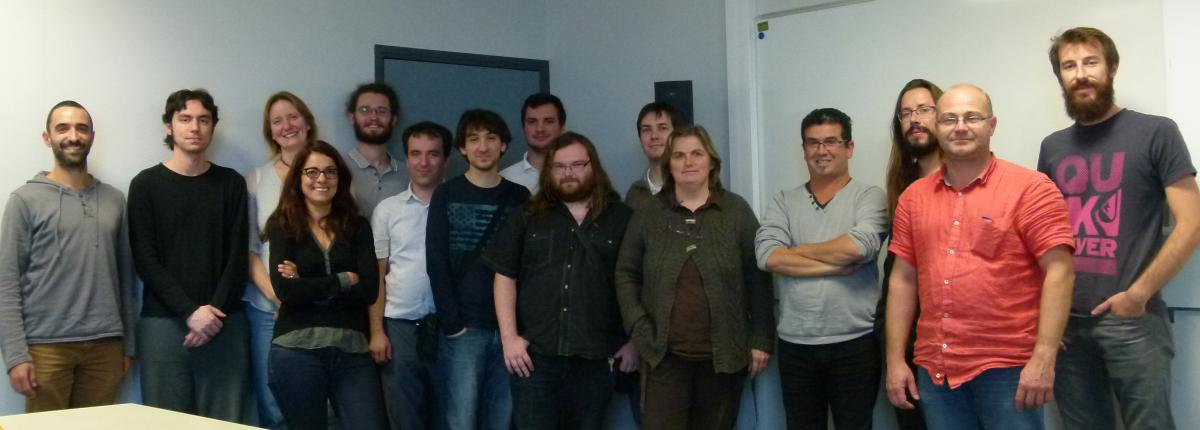
\includegraphics[scale=0.4]{mad.jpg} \end{center}
%\end{quotation}
\newpage
\subsubsection{Qu'est-ce que le Sokoban ?}
Sokoban est un jeu vidéo de puzzle inventé au Japon.
Ce nom désigne un garde d'entrepôt.
Le joueur doit ranger des caisses sur des cases cibles.
Il peut se déplacer dans les quatre directions, et pousser (mais pas tirer) une seule caisse à la fois.
Une fois toutes les caisses rangées (c'est parfois un vrai casse-tête), le niveau est réussi et le joueur passe au niveau suivant, plus difficile, plus complexe et plus élaboré.
L'idéal est de réussir avec le moins de coups possibles (déplacements et poussées).
\newline\newline\newline
\begin{center} 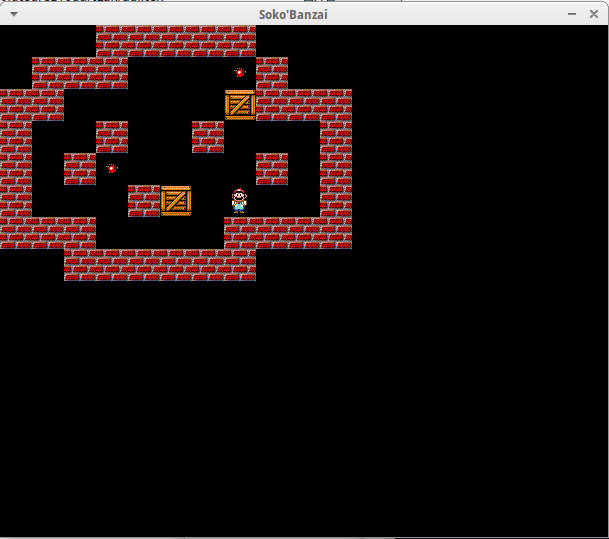
\includegraphics[scale=1]{sokobanzai.png} \end{center}
\newpage



%\newline\newline

%\newpage

\subsection{Analyse du besoin}

\subsubsection{Fonctionnalités à réaliser}
\noindent
\begin{itemize}
\item Implémentation d'un Sokoban en MVP
\item Implémentation d'un algorithme A*
\item Mise en place d'un système de test de différents algorithmes sur le Sokoban
\item Mise en place d'un générateur aléatoire de niveaux de Sokoban
\newline
\end{itemize} 




\subsubsection{Demande initiale}
\noindent
\textbf{Demande sur le MVP :}
\newline\newline
Le code d'un Sokoban sans pattern a été proposé au client mais le client a refusé car le code n'était pas adaptable a ses algorithme.
\newline
Le choix d'implémentation d'un MVP (Modèle Vue Présentateur) a donc été mis en place.
\newline\newline
\textbf{Demande sur le A* :}
\newline\newline
Le projet en l'état a pris du retard mais l'implémentation d'un algorithme de résolution du Sokoban va bientôt être mis en place, le A* sera implémenté avec comme heuristiques une distance euclidienne ou une distance de Manhattan.
\newline\newline
\textbf{Demande sur la mise en place d'un générateur aléatoire de niveaux de Sokoban :}
\newline\newline
La mise en place d'un générateur aléatoire de niveaux de Sokoban n'a pas pu être effectuée.
%

\subsubsection{Le cahier des charges}
\noindent
\textbf{Notre cahier des charges se compose de trois parties :}
\newline
\begin{itemize}
\item Une partie jeu où nous devons essayer de faire un jeu qui soit à la fois léger et qui permette une bonne jouabilité.
\item Une partie interface graphique où nous devons essayer de faire l’interface au graphisme abouti au maximum de nos capacités avec le temps qu'il nous était, afin que le jeu attire l’oeil de toute personne intéressée.
\item Mise en place d'un système de test de différent algorithme sur le Sokoban
\item Une partie intelligence artificielle permettant au personnage de résoudre les différents niveaux de Sokoban tout seul.
\newline
\end{itemize} 


\newpage
\section{Réalisation}
\subsection{interface}
\noindent
\textbf{3 classes principales différentes :}
\newline\newline
\textsc{Vue principale :} 
\newline\newline
Cette classe est directement reliée avec le présentateur, elle représente la vue générale de notre application, en outre, elle possède un "KeyListener" sur notre classe PanneauGrille, permettant d'écouter le déplacement du personnage.
\newline\newline
Notre VuePrincipal instancie un nouveau modele, donc une nouvelle grille par le biais du présentateur lorsque le niveau est terminé. Nous passons ainsi au niveau suivant et la vue se met a jour en fonction du modele. En demande à la vue de la grille de notre classe PanneauGrille de se mettre a jour.
\newline\newline
\textsc{Affichage de la grille de jeu :}
\newline\newline
La classe nommé PanneauGrille est instanciée avec comme paramètre notre grille du modele, puis l'affichage est directement dessinée après un appel à la méthode : « public final void dessiner(Grille grille) » en parcourant la grille, nous récupérerons le contenu de chaque case, par la suite nous instancions une nouvelle VueCase associée a chaques différentes case de la grille, puis chacune des cases de la grille vaut la valeur de l'instance de vue case, enfin nous ajoutons un listener sur cette même instance. Lors de la mise a jour de la vue, il y a un appel à la methode "update" qui supprime tous le contenu de la grille actuel, et redessine la grille la vue correspondant à la grille passée en argument.
\newline\newline
\textsc{Vue des cases :}
\newline\newline
Vue graphique de chaque case de la grille.
Notre classe possède un attribut de classe de type tableau ImageIcon[] appelé "sprite" représentant les sprites des différentes images de cases stocké dans le repertoire "ressources/sprites/" de notre application.
\newline\newline
Notre vue de case est donc instanciée par le biais d’un attribut de type modele.Case associé à son image correspondante dans le tableau des sprites. En effet, il existe un type énumérée dans notre classe modele.Case permettant d’associé le statut d’une case a une image particulière grâce a la méthode java "ordinal()". Nous parcourons les enums en parallèles.
\newline\newline
Notre classe implémentant l’interface « Observer » nous ajoutons a chacune de nos case un observer, en réalité, notre classe VueCases observe la classe modele.Case.
\newline\newline
Nous possédons en conséquence la méthode "public void update(Observable observable, Object object)" qui est appelée quand l'objet observe a change (Nous changeons l’image de la case observée).
\newpage
\subsection{modèle}
\noindent 
%\textbf{Notre modèle possède 8 classes :}
\newline\newline
\textsc{Personnage :}
\newline\newline
Le personnage est instancié dans la classe Grille représentant notre plateau de jeu. Il est définit par ses mouvements et son orientation.
Le personnage possède donc des coordonnées (x, y) qui lui sont propre dans la grille ce qui permet de le situer, nous pouvons ensuite incrémenter ou décrémenter ces coordonnées en fonction du déplacement.
\newline
Par exemple, lorsque nous appuyons sur la flèche directionnelle de droite, nous appellons une fonction aDroite() qui elle-même va appeler la méthode deplacementVers(deltaX, deltaY) où deltaX vaut 0 et deltaY vaut +1, dans laquelle nous avons défini les éléments de façon à ce que le personnage ne puisse aller plus loin que le cadre de jeu, et qu'il ne soit pas en capacité de pousser 2 caisses en même temps.
\newline
La méthode aDroite() va donc appeler la methode deplacementVers(0, +1)incrémenter la coordonné « y », modifier l’orientation du personnage et par la suite assigne dans ses nouvelles coordonnées une nouvelle image associée à son orientation.
De plus la méthode deplacementVers(deltaX, deltaY) va effacer l’ancienne case où était le personnage.
Puis notifie ses changements à la vue par le biais de la méthode notifier(), car la classe Personnage hérite d’Observable.
\newline\newline
\textsc{Grille :}
\newline\newline
La grille est la classe principale du jeu, reliée avec le présentateur.
La méthode principale permet de tester la victoire de l’utilisateur à chaque déplacement du personnage, l’utilisateur gagne lorsqu’il n'y a plus d’objectif et que le personnage n'est pas sur un objectif de la grille.
\newline\newline
testVictoire() : 
\newline\newline
nous testons la valeur binaire d’un booléen égal à true ( donc valant 1 ) ET binaire sur le fait que toutes les cases de la grille soient différentes d’un objectif ET logique d’un personnage sur objectif.
\newline
Dès lors que toutes les valeurs de bits sont égale a 1, la victoire est acquise.
\newline
Une fois la partie terminée, nous initialisons la grille du niveau suivant, et ainsi de suite.
\newline
Cependant, la grille ne peut être instanciée seulement si le niveau a été lu au préalable. En effet notre constructeur principal de la grille est : « public Grille(GestionNiveau gestionNiveau) » où le paramètre « gestionNiveau » nous permet de savoir sur quel numéro de niveau nous sommes.
Nous pouvons ainsi initialiser la grille de jeu d’un niveau de sokoban en utilisant les fichiers .sok de niveau se trouvant dans le répertoire /ressources/niveau/

\begin{center} 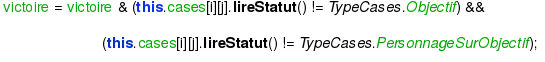
\includegraphics[scale=1]{code1.png} \end{center}
%\newline\newline
\newpage
\noindent
\textsc{GestionNiveau :}
\newline\newline
C'est la classe permettant de lire et de se déplacer dans les différents niveaux du jeu.
Nous utilisons un simple BufferedReader sur notre fichier de niveau .sok lors de l’instanciation de notre classe.
De plus, nous avons la possibilité d’aller au niveau suivant, précédent, ou de se rendre à un niveau voulu passé en paramètre de notre méthode « public void allerAuNiveau(int nbNiveau) ».
\noindent
\newline\newline
\textsc{ChargeurNiveau :}
\newline\newline
La classe qui permet ce chargement s’appelle ChargeurNiveau, celle-ci lit un fichier ".sok" qui est un simple fichier .txt mais appelé .sok pour Sokoban qu’il récupère via la classe Grille et le parse. Dès lors que la variable victoire passe à "true", la méthode partieTermine() est appelée, permettant ainsi d’incrémenter le niveau et d’initialiser la grille sur ce nouveau niveau (ChargeurNiveau charge alors le nouveau niveau).
\newline
Dans Grille la méthode suivante envoie au ChargeurNiveau le niveau qu’il doit lire :
\newline
\begin{center} 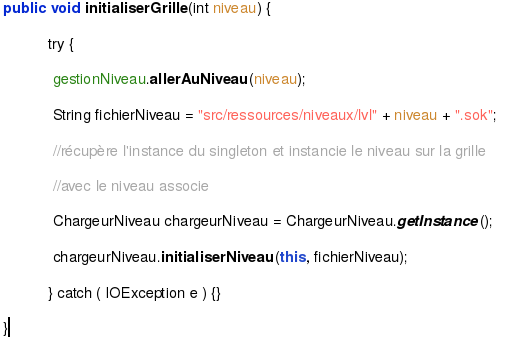
\includegraphics[scale=1]{code2.png} \end{center}
%\newline\newline
\newpage
Le ChargeurNiveau lit le fichier ".sok" indiqué caractère par caractère, jusqu’à ce qu’il rencontre la lettre « A » où il doit s’arrêter. En effet, nous avons récupéré des niveaux pré-fait sur internet d’où l’importance de citer l’Auteur. Nous avons cependant modifié quelques niveaux, par conséquent nous avons dû changé le nom de l’auteur. Quand ChargeurNiveau lit ce fichier il créé une nouvelle « Case(TypeCases statut) » et transforme chaque caractère lu en type énuméré représentant le statut de cette case. Par exemple pour un "\#" il instancie un TypeCase.Mur, un "@"  représente TypeCase.Personnage…
\newline
\begin{center} 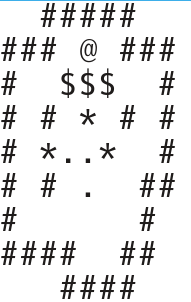
\includegraphics[scale=1]{code3.png} \end{center}
%\newline
Le ChargeurNiveau possède une sous classe « ChargeurNiveauSingleton » représentant notre singleton et possède un attribut d’instance statique qui ne sera chargée en mémoire que lorsque nous y ferons référence pour la première fois.
Celle-ci possède une méthode permettant d'initialiser un niveau sur une grille à l'aide du nom du fichier, en parsant le fichier de niveau. Chaque élément du fichier instancie un certain type de case de notre classe Case en utilisant son type énuméré TypeCases.
\newline\newline
\noindent
\textsc{Case et Personnage :}
\newline\newline
Les classes Case et Personnage correspondent à deux classes distinctes héritant de la classe Observable, elles sont ainsi observées par la vue représentant l'affichage graphique des cases.
\newline
Notre classe Case possède un enum permettant de différencier les divers types de cases, et une case est instanciée par la valeur de son enum où par une case elle même en changeant le statut de celle-ci, pour pouvoir le notifier a son observateur.
\newline
La classe Personnage, n’est en réalité qu’une classe servant a l’instanciation et au déplacement de celui-ci. En effet a chaque keyEvent tapé, le personnage se déplace et le notifie a son observateur, a chaque déplacement l’orientation du personnage est modifié pour permettre un rendu visuel un peu plus réaliste.
\newline\newline
\textbf{Remarque :}
\newline\newline
Au début de notre projet nous voulions que les caisses se déplacent 1 fois sur 10 en glissant d’une case de plus que normalement. Pour cela nous devions mettre en place une interface DeplacementParDefaut, puis une classe DeplacementGlissant qui reproduit un déplacement par défaut avec une chance de faire glisser une caisse d’une case de plus sur un cote ou en face du personnage. Cependant, nos classes de déplacement de sont pas encore fonctionnelle (excepté celle du personnage qui représente un déplacement par défaut).
\newpage
%\subsection{algorithmes}

%\subsection{fonctionnement} 

\subsection{La conception technique} 
\subsubsection{Pattern MVP}
\noindent
\textbf{Modèle :}
\newline\newline
Les classes représentant les données manipulées à travers l'interface utilisateur.
\newline\newline
\noindent
\textbf{Vue :}
\newline\newline
Les classes présentant une vue des données à l'utilisateur.
\newline\newline
\noindent
\textbf{Présentateur :}
\newline\newline
Partie communicant avec les deux autres pour traduire et transmettre les commandes de l'utilisateur envoyée de la vue vers le modèle et pour formater et afficher les données du modèle dans la vue.
\newline
Le principe est de découpler la vue et le modèle, en utilisant le présentateur comme intermédiaire.
\newline\newline
En effet, lorsque l’utilisateur joue a notre jeu il démarre le Présentateur, qui instancie un niveau, puis une grille sur ce niveau et enfin la vue associé à la grille du modèle, a chaque fois que l’utilisateur effectue une action, il modifie le modèle (représentant notre classe Grille dans le Présentateur) suite a quoi, 	le présentateur signale a la vue principale que le modèle a changé, et elle-même va signaler à la vue de notre grille de se modifier en conséquence.
\newline
Dès lors que le modèle indique que la partie est finie (c’est-à-dire victoire de l’utilisateur, changement de niveau, ou réinitialisation du niveau) la vue indique au présentateur de créer un nouveau modèle du niveau en conséquence. 
\newline
Pour l’instant, notre présentateur possède une boucle infinie ne s’arrêtant que si il y a eu victoire de l’utilisateur ou utiliser la méthode « recommencer » permettant de réinitialiser le niveau courant.
\newline
Nous ne gérons pas encore le fait d’aller au niveau suivant/précédent.
\newline\newline
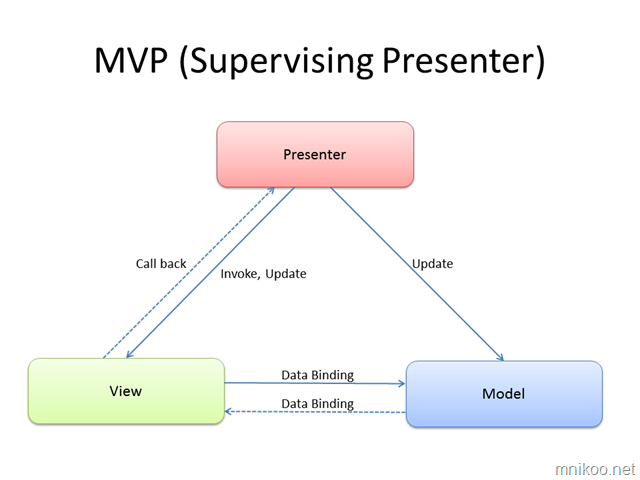
\includegraphics[scale=1]{mvp.png}
\newpage
\subsubsection{Diagramme Modele}

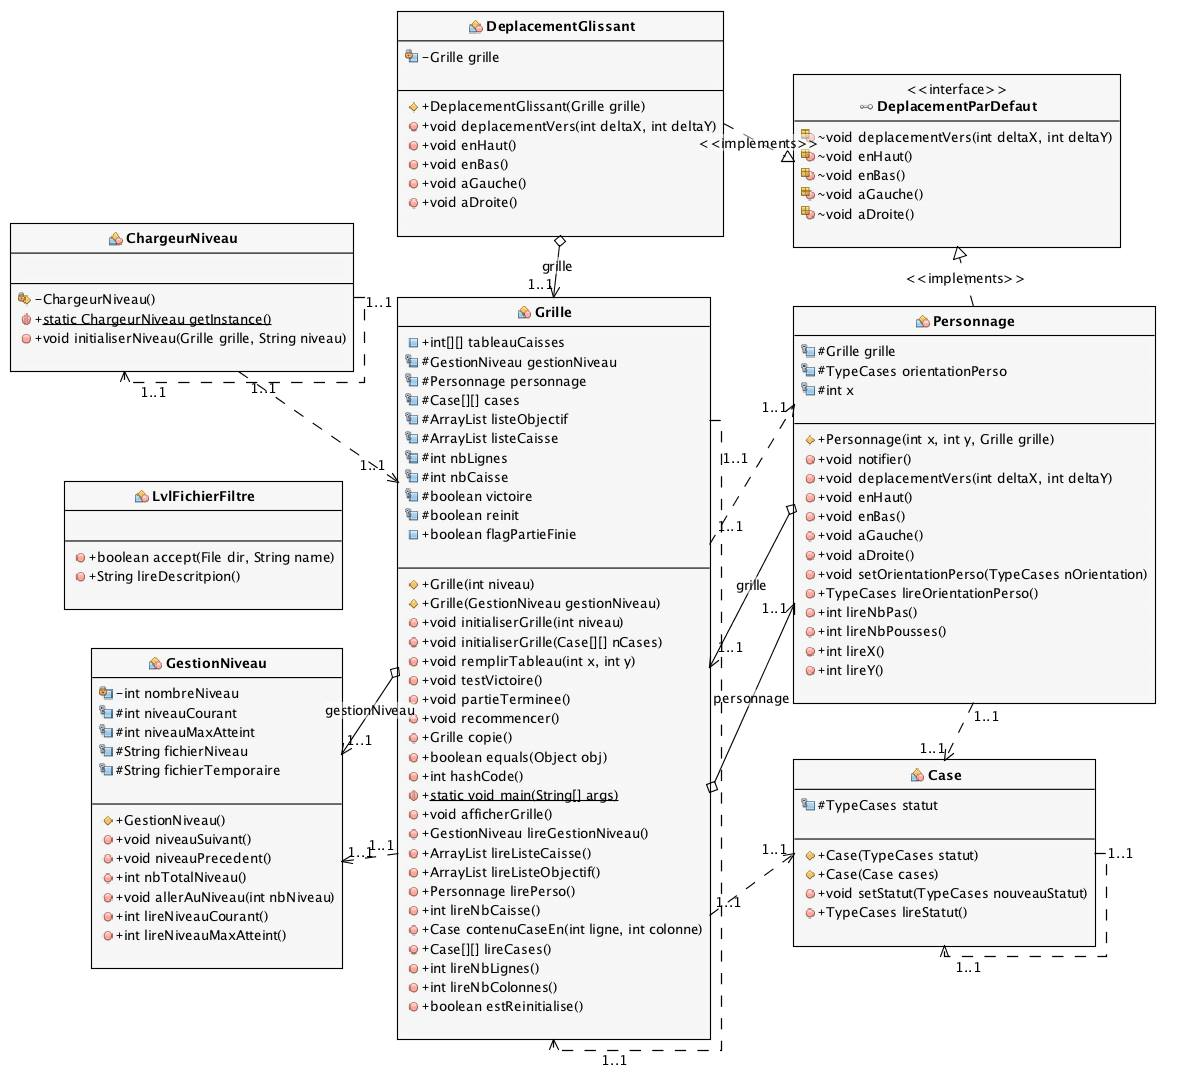
\includegraphics[scale=0.43]{modele2.jpg}
\newpage
\subsubsection{Diagramme Vue}

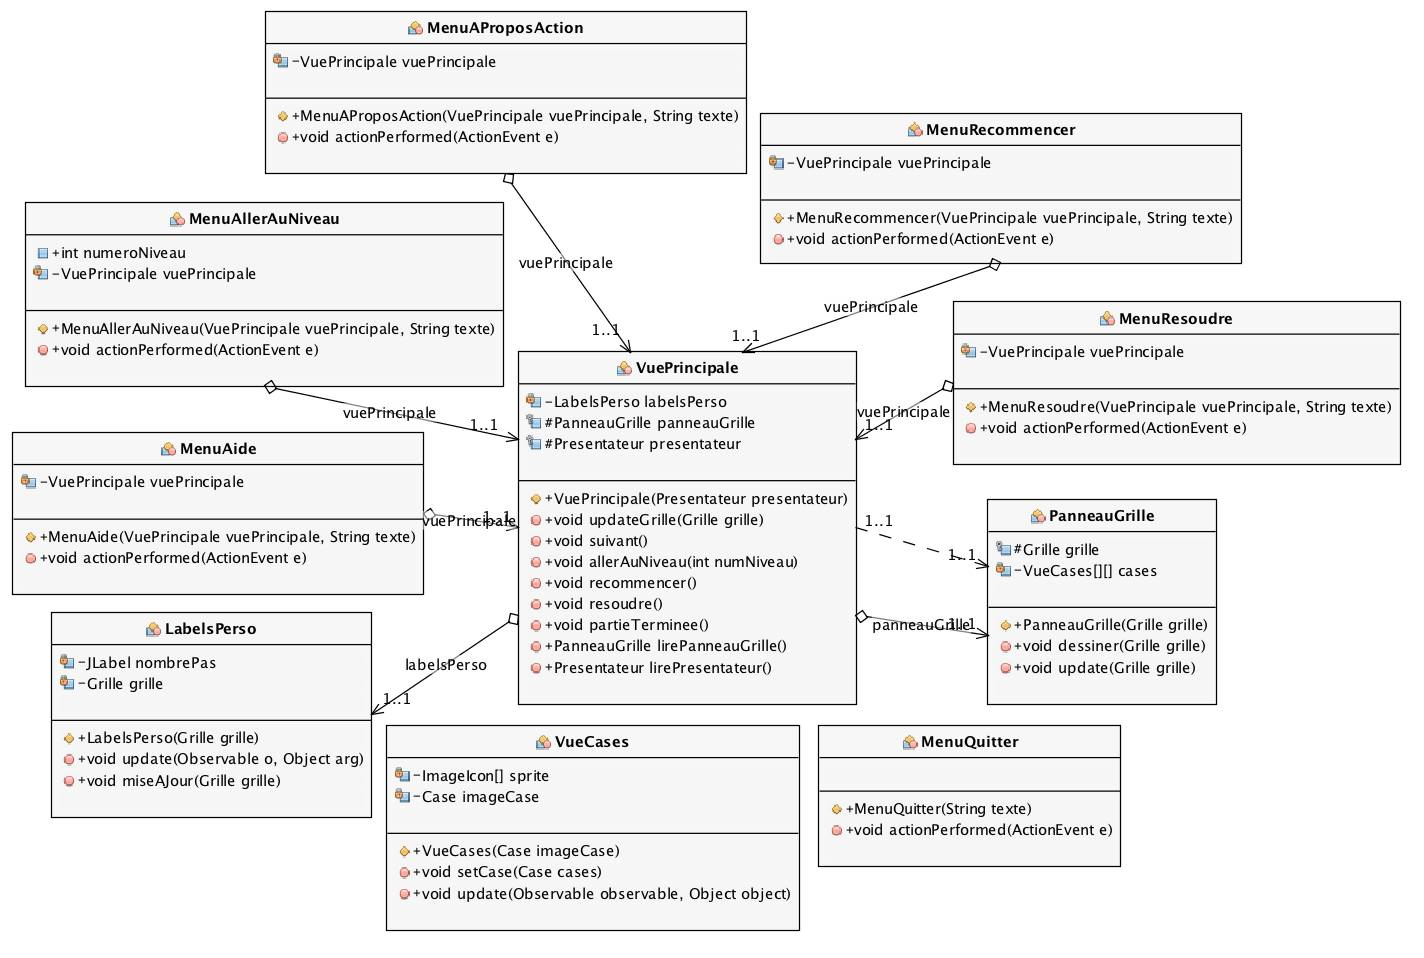
\includegraphics[scale=0.36]{vue2.jpg}
\newpage


%\subsection{Tests sur l'application}
%\noindent

%\newpage
%\subsection{Résultats des tests sur l'application}
%\noindent

%\newpage  
\section{Intelligence Artificielle}
\subsection{Qu'est-ce que l'intelligence artificielle ?}
\subsubsection{Définition}
Le terme « intelligence artificielle », créé par John McCarthy, est souvent abrégé par le sigle "I.A." (ou "A.I." en anglais, pour Artificial Intelligence). 
\newline
Il est défini par l’un de ses créateurs, Marvin Lee Minsky, comme "la construction de programmes informatiques qui s’adonnent à des tâches qui sont, pour l’instant, accomplies de façon plus satisfaisante par des êtres humains car elles demandent des processus mentaux de haut niveau tels que : l’apprentissage perceptuel, l’organisation de la mémoire et le raisonnement critique" Nous y trouvons donc le côté "artificiel" atteint par l'usage des ordinateurs ou de processus électroniques élaborés et le côté "intelligence" associé à son but d'imiter le comportement. 
\newline
Cette imitation peut se faire dans le raisonnement, par exemple dans les jeux ou la pratique des mathématiques, dans la compréhension des langues naturelles, dans la perception : visuelle (interprétation des images et des scènes), auditive (compréhension du langage parlé) ou par d'autres capteurs, dans la commande d'un robot dans un milieu inconnu ou hostile.
Même si elles respectent globalement la définition de Minsky, il existe un certain nombre de définitions différentes de l'IA qui varient sur deux points fondamentaux :
\newline
Les définitions qui lient la définition de l'IA à un aspect humain de l'intelligence, et celles qui la lient à un modèle idéal d'intelligence, non forcément humaine, nommée rationalité.
\newline
Les définitions qui insistent sur le fait que l'IA a pour but d'avoir toutes les apparences de l'intelligence (humaine ou rationnelle), et celles qui insistent sur le fait que le fonctionnement interne du système d'IA doit ressembler également à celui de l'être humain et être au moins aussi rationnel. 
\subsubsection{Historique}

L'origine de l'intelligence artificielle se trouve probablement dans l'article d'Alan Turing "Computing Machinery and Intelligence" (Mind, octobre 1950), où Turing explore le problème et propose une expérience maintenant connue sous le nom de test de Turing dans une tentative de définition d'un standard permettant de qualifier une machine de "consciente".
\newline
Il développe cette idée dans plusieurs forums, dans la conférence "L'intelligence de la machine, une idée hérétique", dans la conférence qu'il donne à la BBC e programme le 15 mai 1951 "Les calculateurs numériques peuvent-ils penser ?" ou la discussion avec M.H.A. Newman, Sir Geoffrey Jefferson et R.B. Braithwaite les 14 et 23 janvier 1952 sur le thème "Les ordinateurs peuvent-ils penser?".
\newline
On considère que l'intelligence artificielle, en tant que domaine de recherche, a été créée à la conférence qui s'est tenue sur le campus de Dartmouth College pendant l'été 1956 à laquelle assistaient ceux qui vont marquer la discipline. 
\newline
Ensuite l'intelligence artificielle se développe surtout aux États-Unis à l'université Stanford sous l'impulsion de John McCarthy, au MIT sous celle de Marvin Minsky, à l'université Carnegie-Mellon sous celle de Allen Newell et Herbert Simon et à l'université d'Édimbourg sous celle de Donald Michie. En France, l'un des pionniers est Jacques Pitrat.
\newpage
\subsection{L'algorithme A *}
L'algorithme de recherche A* (qui se prononce A étoile, ou A star à l'anglaise) est un algorithme de recherche de chemin dans un graphe entre un nœud initial et un nœud final tous deux donnés. De par sa simplicité il est souvent présenté comme exemple typique d'algorithme de planification, domaine de l'intelligence artificielle. L'algorithme A* a été créé pour que la première solution trouvée soit l'une des meilleures, c'est pourquoi il est célèbre dans des applications comme les jeux vidéo privilégiant la vitesse de calcul sur l'exactitude des résultats. Cet algorithme a été proposé pour la première fois par Peter E. Hart, Nils John Nilsson et Bertram Raphael. Il s'agit d'une extension de l'algorithme de Dijkstra de 1959.
\newline\newline
\textbf{Présentation :}
\newline\newline
L'algorithme A* est un algorithme de recherche de chemin dans un graphe entre un nœud initial et un nœud final. Il utilise une évaluation heuristique sur chaque nœud pour estimer le meilleur chemin y passant, et visite ensuite les nœuds par ordre de cette évaluation heuristique. C'est un algorithme simple, ne nécessitant pas de prétraitement, et ne consommant que peu de mémoire.
\newline\newline
\textbf{Intuition :}
\newline\newline
Commençons par un exemple de motivation. Nous nous trouvons à l'intersection A et nous voulons nous rendre à l'intersection B dont nous savons qu'elle se trouve au nord de notre position actuelle. Pour ce cas classique, le graphe sur lequel l'algorithme va travailler représente la carte, où ses arcs représentent les chemins et ses nœuds les intersections des chemins.
\newline
Si nous faisions une recherche en largeur comme le réalise l'algorithme de Dijkstra, nous rechercherions tous les points dans un rayon circulaire fixe, augmentant graduellement ce cercle pour rechercher des intersections de plus en plus loin de notre point de départ. Ceci pourrait être une stratégie efficace si nous ne savons pas où se trouve notre destination, comme la police recherchant un criminel en planque.
\newline
Cependant, c'est une perte de temps si noud connaîssons plus d'informations sur notre destination. Une meilleure stratégie est d'explorer à chaque intersection la première directement qui va vers le nord, car le chemin le plus court est la ligne droite. Tant que la route le permet, nous continuons à avancer en prenant les chemins se rapprochant le plus de l'intersection B. Certainement devrons-nous revenir en arrière de temps en temps, mais sur les cartes typiques c'est une stratégie beaucoup plus rapide. D'ailleurs, souvent cette stratégie trouvera le meilleur itinéraire, comme la recherche en largeur le ferait. C'est l'essence de la recherche de chemin A*.
Un labyrinthe simple, où l'algorithme A* ne sera pas très efficace
\newline
Toutefois, comme pour tous les algorithmes de recherche de chemin, leur efficacité dépend fortement du problème que nous souhaitons résoudre (c'est-à-dire : du graphe). Ainsi l'algorithme A* ne garantit pas de trouver un itinéraire plus rapidement qu'un autre algorithme, et dans un labyrinthe, la seule manière d'atteindre la destination pourrait être à l'opposé de la position de la destination, et les nœuds les plus proches de cette destination pourraient ne pas être sur le chemin le plus court, ce qui peut coûter beaucoup de temps de calcul.
\newline\newline
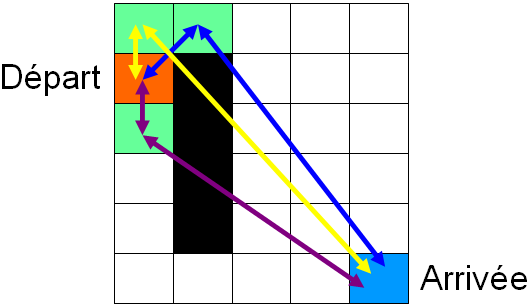
\includegraphics[scale=0.3]{astar.png}

\subsection{Notre IA}
Nous possédons un package nommé « ia », contenant certaines classes abstraites ou interfaces, permettant ainsi d’implémenter n’importe quel type d’algorithme à n’importe quel type de problème. En effet, après avoir discuté avec notre client, nous avons implémenté un code en types génériques.
\newline\newline 
Cependant, la gestion d’exception n’ayant pas encore était implémentée, faute de temps, nous supposerons que l’utilisateur ne se trompe pas de type pour que la compilation ne retourne pas d’erreurs.
\newline\newline 
Concernant les interfaces génériques, nous possédons:
\newline
\begin{itemize}
\item HeuristiqueAbstrait <E>
\item ProblemeAbstrait <E, A>
\item AlgorithmeAbstrait <E, A>
\newline
\end{itemize}
%\newline\newline
Dans notre cas : 
\newline
\begin{itemize}
\item Le type E représente une grille, un état du jeu.
\item Le type A représente une action applicable au jeu, un déplacement du personnage.
\newline
\end{itemize}
%\newline
\noindent
\textbf{HeuristiqueAbstrait <E> :}
\newline\newline
Interface permettant d’ajouter une nouvelle heuristique admissible à appliquer sur un état E. Nous avons pour l’instant 2 méthodes heuristiques. Une permettant de calculer la distance Manhattan entre une caisse et un objectif, et une autre permettant de calculer la distance Manhattan entre le personnage et une caisse.
\newline\newline
\noindent
\textbf{ProblemeAbstrait <E, A> :}
\newline\newline
Définit 4 méthodes, dont 3 sont des accesseurs permettant de :
savoir si un état E est terminal (victoire du personnage.)
faire la lecture de l’état courant du problème connaitre la liste des actions de l’état courant du problème.
\newline
Sa 4ème méthode est « E successeur(E état, A action) », comme son nom l’indique, elle renvoie l’état successeur d’un état donné ayant une certaine action effectuée sur celui-ci.
\newline\newline
\noindent
\textbf{AlgorithmeAbstrait <E, A> :}
\newline\newline
Possède une unique méthode
\newline
"ArrayList<E> resoudre(ProblemeAbstrait <E, A> probleme, HeuristiqueAbstrait<E> heuristique);"
\newline
qui permet de résoudre un problème donné avec une certaine heuristique, à condition que cette heuristique soit « admissible ». 
\newpage
\noindent
\textsc{Passons maintenant aux classes concrètes de notre implémentation d’intelligence artificielle;
Nous possédons 4 classes concrètes, et 1 type énuméré fortement typé :}
\noindent
\newline\newline
\textbf{ActionSokoban :}
\newline\newline
Celle-ci est la plus simple, c’est notre type énuméré qui représente tout simplement les 4 actions possibles d’un personnage sur une grille à savoir, les 4 déplacements : Haut, Bas, Gauche et Droite.
\noindent
\newline\newline
\textbf{ProblemeSokoban :}
\newline\newline
Cette classe, implémente l’interface ProblemeAbstrait <Grille, ActionSokoban>, un problème s’instancie simplement à l’aide d’une grille, et lors de son instanciation, celui-ci créé un EnumSet « actions » de toutes les valeurs contenues dans le type énuméré « ActionSokoban ».
\newline
Puis affecte à la variable « listeActions » étant une List<ActionSokoban> une nouvelle ArrayList de « actions » :
\newline\newline
"EnumSet < ActionSokoban > actions = EnumSet.allOf( ActionSokoban.class );"
\newline
\indent\indent "ProblemeSokoban.listeActions = new ArrayList(actions);"
\newline\newline
Cette classe redéfinit la méthode principale appelée « successeur », cette méthode prend en argument une grille à un certain état, et une action. 
\newline\newline
Lors d’un appel à « successeur » la grille passée en paramètre est copiée pour ne pas la modifier directement, puis applique l’action du personnage sur la copie de la grille et retourne la copie modifiée. Cette méthode permet donc de passer d’un état à un autre sans modifier l’état initial.
\newline 
De plus, ProblemeSokoban redéfinit la méthode permettant de savoir si une grille est terminale ou non (si le personnage à réussi à placer toutes les caisses sur les objectifs.).
\newline\newline
\noindent
\textbf{HeuristiqueSokoban :}
\newline\newline
Notre classe qui implémente HeuristiqueAbstraite, nous avons décidé d’utiliser une heuristique permettant de connaitre la plus courte distance Manhattan entre (le personnage et les caisses) additionnée à la plus courte distance Manhattan entre (les caisses et les objectifs). 
\newline\newline
La distance Manhattan représente le nombre de cases, en horizontal et en vertical entre la source et la destination. 
\newline
Malheureusement, nos heuristique ne sont pas réellement au point. 
\newline\newline
En effet dès lors qu’il existe plusieurs caisses (donc plusieurs objectifs) sur une grille, notre heuristique prend en compte seulement la dernière caisse traitée et le dernier objectif, nous n’arrivons pas à stocker toutes les valeurs de coordonnées (x,y) des différentes caisses et objectifs présents sur la grille.
\newpage 
\noindent
\textbf{GrilleAvecValeur :}
\newline\newline
Cette classe n’est en réalité rien de plus qu’une grille « possède un attribut Grille grille », avec en plus des valeurs utilisées dans les différents algorithme de recherche de plus court chemin a savoir la fonction "g" où " g(etatCourant)" est le coût du meilleur chemin connu pour atteindre etatCourant depuis l'état initial; à savoir que comme nous avons un terrain toujours identique, le coût d’un déplacement du personnage est constant et vaut 1, donc pour passer d’une grille a une autre en faisant un déplacement de personnage nous faisons simplement "g+1". 
\newline\newline
La seconde valeur est nommée "h" et représente la fonction heuristique (prédictions) permet d’évaluer un coût vers la destination INFERIEUR au coût réel (encore inconnu).
\newline
A ce titre, A* est un algorithme optimiste.
\newline
Notre "h" représente donc un entier,  d’estimation des distances entre le sommet initial et le sommet terminal.
\newline
Donc pour trouver la valeur de la variable "h" il faudra additionner la valeur de retour des deux méthodes de calcul de distance d’une instance de notre classe vu précédemment "HeuristiqueSokoban" sur une grille à un moment donné. 
\newline\newline
Cette classe servant notamment de référence de comparaison, elle implémente donc l’interface "Comparable" de l’API Java, nous redéfinissons donc sa méthode "compareTo(Object obj)". 
\newline\newline
Nous comparons donc deux grilles avec valeurs entre la valeur de l’heuristique de la grille actuel avec celle de la grille « obj » passée en argument, si les valeurs des deux « h » sont égales nous retournons 0, si la valeur du « h » de la grille actuel est supérieure à la grille « obj » nous retournons 1, sinon nous retournons -1.
\newline\newline
Ceci nous permet de trier l’ordre de priorité des différentes GrilleAvecValeur dans une PriorityQueue de l’algorithme A*.
\newline\newline
A propos de la PriorityQueue, nous avons eux beaucoup de problème sur le fait que la PriorityQueue par défaut compare l’égalité des pointeurs, or nous voulions comparer l’égalité de deux grille, cet-à-dire l’égalité des positions du personnage et des caisses.
\newline\newline
Nous avons donc du redéfinir les méthodes "equals(Object obj)" et "hashCode()" de la class "Object" dont toutes les classes hérite par défaut.
\newline\newline 
La méthode "equals(Object obj)" test si l’objet passé en argument est une instance de GrilleAvecValeur, si l'argument n'est pas une instance de GrilleAvecValeur, nous retournons "False;" sinon nous retournons la valeur du booléen de l’attribut grille actuel "equals" (appel à la méthode "equals(Object obj)" redéfinit dans la classe Grille du modèle, d’où l’intérêt du cast pour empêcher une exception)  à l’attribut "grille" de la grille avec valeur passé en paramètre : 
\newline\newline    
"return this.grille.equals( ((GrilleAvecValeur) obj).grille );"
\newline\newline
Puis la méthode "hashCode()", nous hashons simplement l’attribut this.grille car seulement celui-ci doit être unique : hash = 29 * hash + Objects.hashCode(this.grille); où hash vaut initialement 5.
\newpage
\noindent
\textbf{Aetoile :}
\newline\newline
Passons maintenant a notre classe principale de l’algorithme de résolution du plus court chemin, l’algorithme A étoile (A star).
\newline\newline
Celui-ci implémente donc l’interface "AlgorithmeAbstrait <E, A>" et s’instancie à l’aide d’un état E, et d’une List<A> où l’état E est une grille, et la liste<A> est la ArrayList d’ActionSokoban vu précédemment.
\newline\newline 
Notre classe possède donc deux accesseurs : un sur la grille et un sur la liste d’action, et redéfinit la méthode considéré comme principale d’ "AlgorithmeAbstrait" nommée 
\newline\newline
"public ArrayList<E> resoudre(ProblemeAbstrait<E, A> probleme, HeuristiqueAbstrait<E> heuristique)".
\newline\newline
Cette méthode retourne une ArrayList<E> qui est en fait une liste contenant tous les sommets visitées (représente notre liste ferme) si il existe une solution et retourne "null" sinon, cela signifie qu’il n’existe pas de chemin possible entre la source et l’état terminal.
\newline\newline
La méthode de résolution maintient deux listes différentes.
\newline\newline
Nous avons choisis d’implémenter une file à priorité dite "ouverte" de type PriorityQueue, qui représente les états à explorer, puis une liste doublement chainée dite "ferme" de type LinkedList qui représente ici les états visités considéré prioritaire par la PriorityQueue.
\newline\newline
Premièrement, nous instancions un état initial appelé "etatInitial", un état source, qui représente l’état courant du problème et non la grille de départ instancié lors du démarrage d’un niveau. 
\newline\newline
Cela permet en effet à un joueur lorsqu’il s’est déjà déplacé, de demander un "indice" à l’algorithme permettant à l’utilisateur de savoir si oui ou non il existe une solution à partir de l’état de la grille sur laquelle il se trouve. 
\newline\newline	
Ensuite, nous instancions une grille avec valeur sur la grille de l’état initial précédent, avec un coup "g" de 0, et appelons "h" la valeur où: 
\newline\newline
"int h = heuristique.distanceManhattanPersonnageCaisse((E) etatInitial) ) 
\newline
+ ( heuristique.distanceManhattanCaisseObjectif((E) etatInitial);".
\newline\newline
Puis nous ajoutons cette grille avec valeur à la liste ouverte.
\newline\newline
Nous commencons la boucle de recherche, tant que la file à priorité n’est pas vide, nous récupèrons la tête de liste, appelons le "etatCourant" il représente l’état avec la fonction F minimale, cet-à-dire avec la somme de "g" et de "h" la plus petite.
\newline\newline
Nous supprimoms etatCourant de la liste ouverte et nous l’ajoutons à la liste ferme.
\newpage
\noindent
Nous testons si le problème de l’état courant est terminal :
\newline\newline
Si oui : 
\newline\newline
Nous récupèrons la dernière valeur de la liste ferme et nous l’assignons dans une variable de type Grille appelons le "noeudCourant", nous le supprimons de la liste, puis nous l’ajoutons à l’ArrayList "chemin", cette liste nous permettra plus tard de reconstruire le chemin de la source a l’état final.
\newline\newline
Nous parcourons la liste ferme des états visités et tant que "noeudCourant" est différents de l’etatInitial nous assignons à "noeudCourant" la dernière valeur de la liste ferme et nous la supprimons, nous ajoutons ensuite « noeudCourant » dans la liste "chemin".
\newline\newline
Sinon :
\newline\newline 
Pour chaque actions du problème qui sont applicable à l’état courant, nous génèrons les 4 successeurs de l’état courant a l’aide de la méthode « successeur » de la classe ProblemeSokoban. Ensuite nous mettons à jour notre heuristique en calculant les nouvelles distances sur les 4 états successeurs.
\newline\newline
Nous incrémentons la fonction "g" de 1 puisque nous avons un coût uniforme peut importe le déplacement.
\newline\newline
Puis, nous instancions 4 nouvelles grilles avec valeur en prenant en paramètre les grilles successeurs, les nouvelles valeur de  "g" et "h".
\newline\newline
Enfin nous réalisons plusieurs tests, d’abord si une des grilles avec valeur successeurs est égale a l’état courant, nous continuons. Nous vérifions que la liste ouverte et la liste ferme ne contiennent pas un des états successeurs ( ici, comme vu précédemment, nous ne comparons pas les pointeurs, mais bel et bien les positions du personnage et des caisses ! ) nous assignons à la fonction "g" de la grille avec valeurs successeurs le nouveau "g".
\newline\newline
Et nous ajoutons ce successeur à la liste ouverte.
\newline\newline
Sinon, si la valeur de la fonction "g" du successeurs est supérieure au nouveau "g", alors nous assignons au "g" du successeur la nouvelle valeur, puis nous vérifions que la liste ferme contient bien cet état successeur, nous le supprimons de la liste ferme, et nous l’ajoutons à la liste ouverte.
\newline\newline
Après tout cela, si l’algorithme ne trouve pas de solution, c’est qu’il n’y en a pas.
\newpage
\subsection{Diagramme IA}
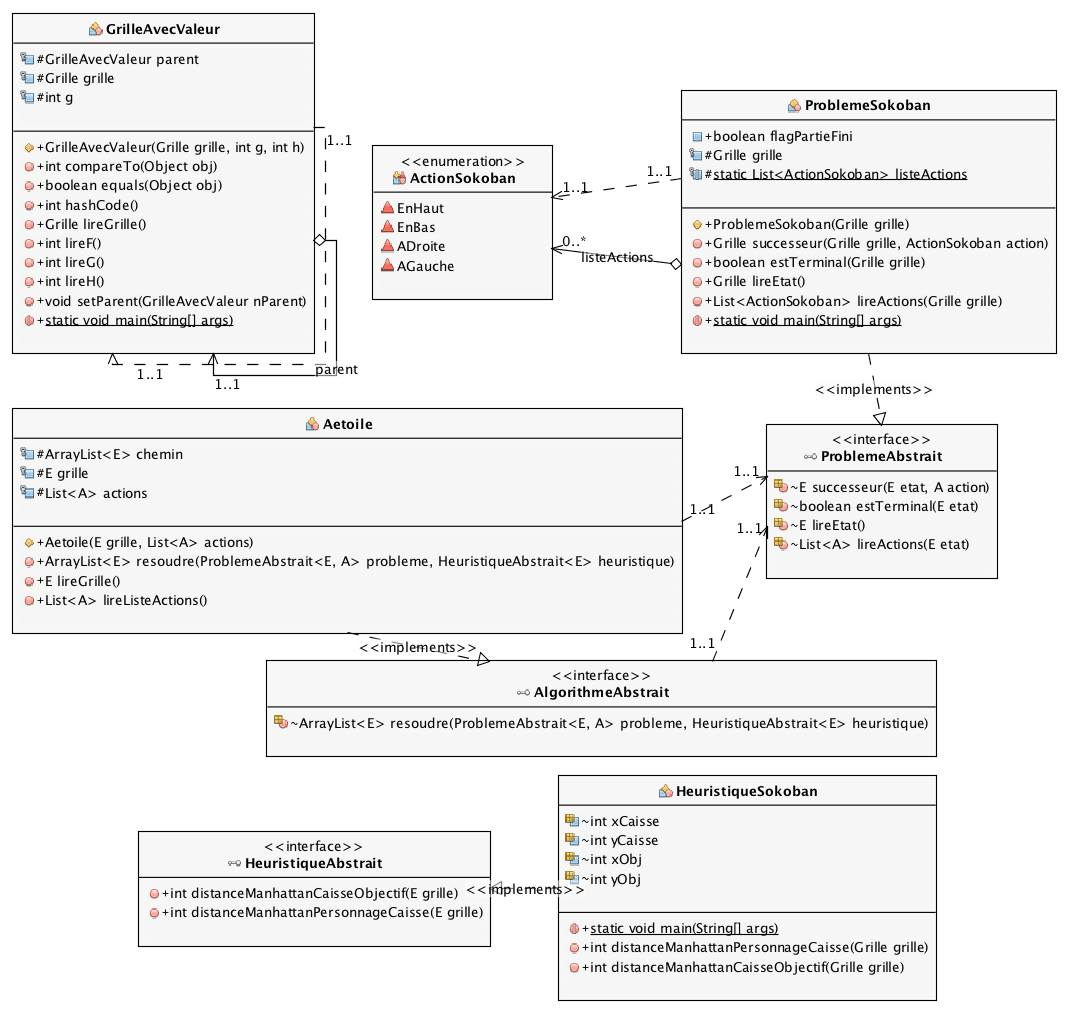
\includegraphics[scale=0.46]{ia2.jpg}
\newpage
\section{Description du déroulement} 
\subsection{Grandes étapes et plannings}
\begin{center} 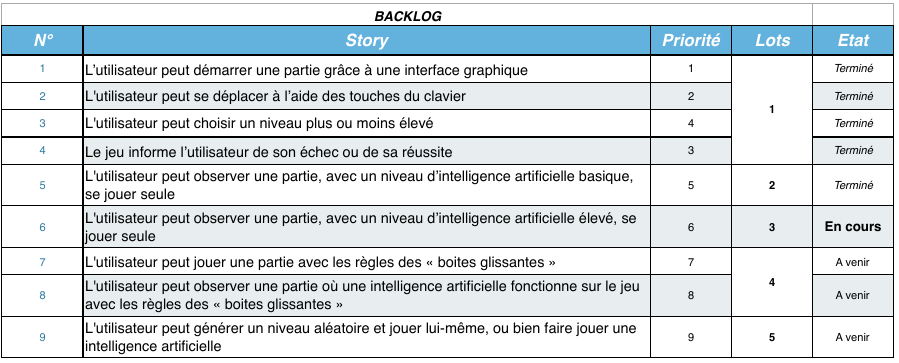
\includegraphics[scale=0.7]{backlogfinal.png} \end{center}

\subsection{Idées proposées et rejetées}
La mise en place d'un générateur aléatoire de niveaux de Sokoban pour la dernière partie étant considérée comme optionnelle, sera sûrement absente du projet final.

\subsection{Problèmes rencontrés et solutions apportées}
Dans la mise en place initial du projet le client nous a proposé de récupérer un code source sur internet, mais il s'est avéré être très mal codé et n'avait pas de pattern MVP implémenté.
\newline
Nous avons donc recommencé tous le projet et pris du retard sur le planning initial.


\subsection{Gestion du projet : organisation et répartition des tâches}
\subsubsection{Forge SVN}

Il s’agit d’un système permettant de sauvegarder les différentes versions du programme.
\newline
 Il permet aussi de suivre l’évolution et les modifications effectuées par un autre utilisateur. Ce système comprend de nombreuses autres fonctionnalités, comme par exemple de faire des demandes aux autres utilisateurs du projet.
\newline
C’est donc un excellent moyen de gestion de projets de groupe.
\subsubsection{Organisation et répartition des tâches}
Avant d’avoir commencé à répartir les tâches, nous  nous sommes d’abord fixé les objectifs que nous avions décidé d'atteindre bien qu’ils n'aient pas tous été atteints.
\newline\newline  
Nous avons fait une répartition selon les différents modules, leurs complexités, et les différentes compétences de chacun.
\newline\newline  
Chacun de nous devait s’occuper d’une ou deux parties, indépendamment les unes des autres.
\newpage
\section{Bilan et Conclusion}
Notre projet fut très intéressant à mettre en place et notre équipe a dans l'ensemble bien fonctionnée.
\newline\newline
Du point de vue technique, ce projet nous a permis d'enrichir nos connaissances sur le java et l'intelligence artificielle et nous a fait découvrir des outils très intéressants  qui se sont avérés très utiles pour la conception et la réalisation du projet.
\newline\newline
Nous avons ainsi pu développer notre technique de recherche d'informations ainsi que notre esprit d'initiative et notre esprit d'équipe.
%\newline\newline
%Notre souhait maintenant est de pouvoir continuer à développer ce projet %et enfin de le voir aboutir, avec bien sur, l'aimable autorisation de nos %professeurs et de l'Université de Caen.
\newpage
\section{Sources et Documentations}
\noindent
\newline\newline
https://www.greyc.fr/fr/mad 
\newline\newline
http://www.gamedev.net/page/index.html
\newline\newline
http://www.redblobgames.com/pathfinding/a-star/implementation.html
\newline\newline
https://docs.oracle.com/javase/7/docs/api/

\end{document}

